% -*- TeX-engine: xetex; eval: (auto-fill-mode 0); eval: (visual-line-mode 1); -*-
% Compile with XeLaTeX

\documentclass[11pt]{article}
%%%%%%%%%%%%%%%%
% Packages
%%%%%%%%%%%%%%%%

\usepackage[top=1cm,bottom=1cm,left=1.5cm,right= 1.5cm]{geometry}
\usepackage[parfill]{parskip}
\usepackage{graphicx, fontspec, xcolor,multicol, enumitem, setspace}
\DeclareGraphicsRule{.tif}{png}{.png}{`convert #1 `dirname #1`/`basename #1 .tif`.png}

%%%%%%%%%%%%%%%%
% No page number
%%%%%%%%%%%%%%%%

\pagestyle{empty}

%%%%%%%%%%%%%%%%
% User defined colors
%%%%%%%%%%%%%%%%

% Pantone 2015 Spring colors
% http://iwork3.us/2014/09/16/pantone-2015-spring-fashion-report/
% update each semester or year

\xdefinecolor{custom_blue}{rgb}{0, 0.70, 0.79} % scuba blue
\xdefinecolor{custom_darkBlue}{rgb}{0.11, 0.31, 0.54} % classic blue
\xdefinecolor{custom_orange}{rgb}{0.97, 0.57, 0.34} % tangerine
\xdefinecolor{custom_green}{rgb}{0.49, 0.81, 0.71} % lucite green
\xdefinecolor{custom_red}{rgb}{0.58, 0.32, 0.32} % marsala

\xdefinecolor{custom_lightGray}{rgb}{0.78, 0.80, 0.80} % glacier gray
\xdefinecolor{custom_darkGray}{rgb}{0.54, 0.52, 0.53} % titanium

%%%%%%%%%%%%%%%%
% Color text commands
%%%%%%%%%%%%%%%%

%orange
\newcommand{\orange}[1]{\textit{\textcolor{custom_orange}{#1}}}

% yellow
\newcommand{\yellow}[1]{\textit{\textcolor{yellow}{#1}}}

% blue
\newcommand{\blue}[1]{\textit{\textcolor{blue}{#1}}}

% green
\newcommand{\green}[1]{\textit{\textcolor{custom_green}{#1}}}

% red
\newcommand{\red}[1]{\textit{\textcolor{custom_red}{#1}}}

%%%%%%%%%%%%%%%%
% Coloring titles, links, etc.
%%%%%%%%%%%%%%%%

\usepackage{titlesec}
\titleformat{\section}
{\color{custom_blue}\normalfont\Large\bfseries}
{\color{custom_blue}\thesection}{1em}{}
\titleformat{\subsection}
{\color{custom_blue}\normalfont}
{\color{custom_blue}\thesubsection}{1em}{}

\newcommand{\ttl}[1]{ \textsc{{\LARGE \textbf{{\color{custom_blue} #1} } }}}

\newcommand{\tl}[1]{ \textsc{{\large \textbf{{\color{custom_blue} #1} } }}}

\usepackage[colorlinks=false,pdfborder={0 0 0},urlcolor= custom_orange,colorlinks=true,linkcolor= custom_orange, citecolor= custom_orange,backref=true]{hyperref}

%%%%%%%%%%%%%%%%
% Instructions box
%%%%%%%%%%%%%%%%

\newcommand{\inst}[1]{
\colorbox{custom_blue!20!white!50}{\parbox{\textwidth}{
	\vskip10pt
	\leftskip10pt \rightskip10pt
	#1
	\vskip10pt
}}
\vskip10pt
}

%%%%%%%%%%%%%%%%
% Timing
%%%%%%%%%%%%%%%%

% 15-20 minutes

%%%%%%%%%%%%%%%%
% Sakai link for course
%%%%%%%%%%%%%%%%

% UPDATE FOR OWN COURSE
% LINK TO ASSIGNMENTS TOOL IN SAKAI

\newcommand{\Sakai}[1]
{\href{https://sakai.duke.edu/portal/site/ba0d1c18-ba55-473f-9d70-b6a1f9559bbe/page/9870858b-a1a9-481e-8497-8a6ffe9e5be2}{Sakai}}

%%%%%%%%%%%
% App Ex number    %
%%%%%%%%%%%

% DON'T FORGET TO UPDATE

\newcommand{\appno}[1]
{5.3}

%%%%%%%%%%%%%%
% Turn on/off solutions       %
%%%%%%%%%%%%%%

% Off
\newcommand{\soln}[1]{
\vskip5pt
}

%% On
%\newcommand{\soln}[1]{
%\textit{\textcolor{custom_darkGray}{#1}}
%}

%%%%%%%%%%%%%%%%
% Document
%%%%%%%%%%%%%%%%

\begin{document}
\fontspec[Ligatures=TeX]{Helvetica Neue Light}

Dr. \c{C}etinkaya-Rundel \hfill Data Analysis and Statistical Inference \\

\ttl{Application exercise \appno{}: \\
Chi-square testing}

\inst{Submit your responses on \Sakai{}, under the appropriate assignment. Only one submission per team is required. One team will be randomly selected and their responses will be discussed.}

\section*{Basketball and presidential vote in NC}

Public Policy Polling surveyed  849 registered North Carolina voters from February 24th to 26th, 2015. The full report on the poll results can be found at \url{http://www.publicpolicypolling.com/pdf/2015/PPP_Release_NC_30515.pdf}. We are going to focus on responses to the following questions:

\begin{itemize}
\item Who will you be rooting for in the Duke-UNC basketball game next month? (Remember this survey was before the Duke-UNC game)
\item In the last presidential election, did you vote for Barack Obama or Mitt Romney?
\end{itemize}

\textbf{Part 1:}

\begin{enumerate}

\item First let's take a look at the following table of vote distribution from the report linked above:

\begin{center}
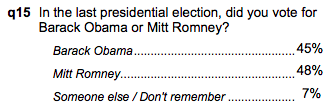
\includegraphics[width=0.4\textwidth]{pp_pres}
\end{center}

According to these results, how many people in the sample voted for Obama, how many for Romney, and how many for others or don't remember?

\item We want to evaluate if NC vote distribution is different than the national outcome (51\% Obama, 47\% Romney, 2\% Other). What test would be appropriate?

\item Calculate the expected counts under the assumption of the null hypothesis of this test being true.

\end{enumerate}

[For the sake of time we'll not complete the test in class, but it's strongly recommended that you complete it on your own.]

\textbf{Part 2:}

\begin{enumerate}[resume]

\item The following table is also from the report linked above. 

\begin{center}
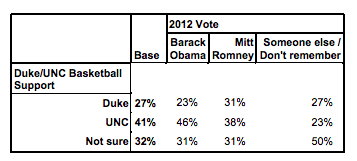
\includegraphics[width=0.4\textwidth]{pp_basket_pres}
\end{center}

Fill in the contingency table of \textbf{counts} below based on these tables. Note that the rest of your responses depend on accurately falling in this table. Please ask questions if you are not sure / get stuck. Hint: You'll need to use

\begin{center}
\begin{tabular}{r | l | l | l | l}
				& Barack Obama	& Mitt Romney	& Other / Don't remember	& Total \\
\hline
\hline
Duke			& *				& 			&					&  \\
\hline
UNC				& 				& 			& 					&  \\
\hline
Not sure			& 				& 			& 					&  \\
\hline
\hline
Total				& 				& 			& 					& 849 \\
\end{tabular}
\end{center}

\item We want to evaluate whether college basketball allegiance of NC residents is associated with how they voted in the 2012 presidential election. What type of test is most appropriate? Explain your reasoning.

\item What are the hypotheses?

\item Calculate the \textbf{expected} number of those who voted for Barack Obama who support Duke.

\item Assuming that all other expected counts are high enough, check if the conditions for inference are met.

\item Calculate the contribution of the ``Duke and voted for Barack Obama" cell (the one with the asterisk in the table above) to the test statistic.

\item The test statistic is given as 17.7161. Calculate the p-value.

\item What is the conclusion of the hypothesis test?

\end{enumerate}

This analysis completed in R can be found at \url{https://stat.duke.edu/courses/Spring15/sta101.001/post/app/basket_pres.html}.

%

\end{document}